\section{Introduction}
\label{sec:introduction}

Wavetable oscillators store one period of a waveform and wrap the read pointer when it reaches the end of the table.
If the first and last samples disagree ($x[0]\neq x[L-1]$), that wrap is a hard discontinuity.
Under cyclic playback it becomes a click that repeats at the fundamental, with a broadband spectrum locked to pitch.
The same geometry appears whenever a short loop is tiled for listening or for objective scoring.

We treat the task as \emph{cycle-local seam restoration}: edit a neighborhood of the wrap---and optionally a small residual cell over the period---so that multi-period playback matches an ideal reference that never opens the wrap cliff.
Agreement is scored by a discontinuity-weighted blend $R_{\mathrm{blend}}$ (seam fidelity vs the ideal, plus mid-cycle identity vs the cracked engine) under a latency-aware objective $J$.

Figure~\ref{fig:intro-sine} shows one hard sine-wrap case from the frozen holdout (same \texttt{make\_batch} tile, seed~\texttt{20260719}).
Four roles must stay distinct:
(a)~ideal sibling $r^{\star}$ (cliff withheld; scoring target, not a method);
(b)~no-bake / cracked engine $x$ after the open-wrap cliff ($R\approx 0.950$ vs $r^{\star}$);
(c)~DualCosine classical end-fade on that tile ($R\approx 0.603$ on this severe cliff);
(d)~Ours / DenoiseOpt favorite bake (\texttt{champion\_iter\_000235}, tile $R\approx 0.9917$).
Panels~(e)--(f) show the modulation residual and a seam zoom.
No-bake is not the ideal.
DualCosine is one classical row and, separately, a PPO advantage baseline (Section~\ref{sec:methods}).

\begin{figure*}[t]
  \centering
  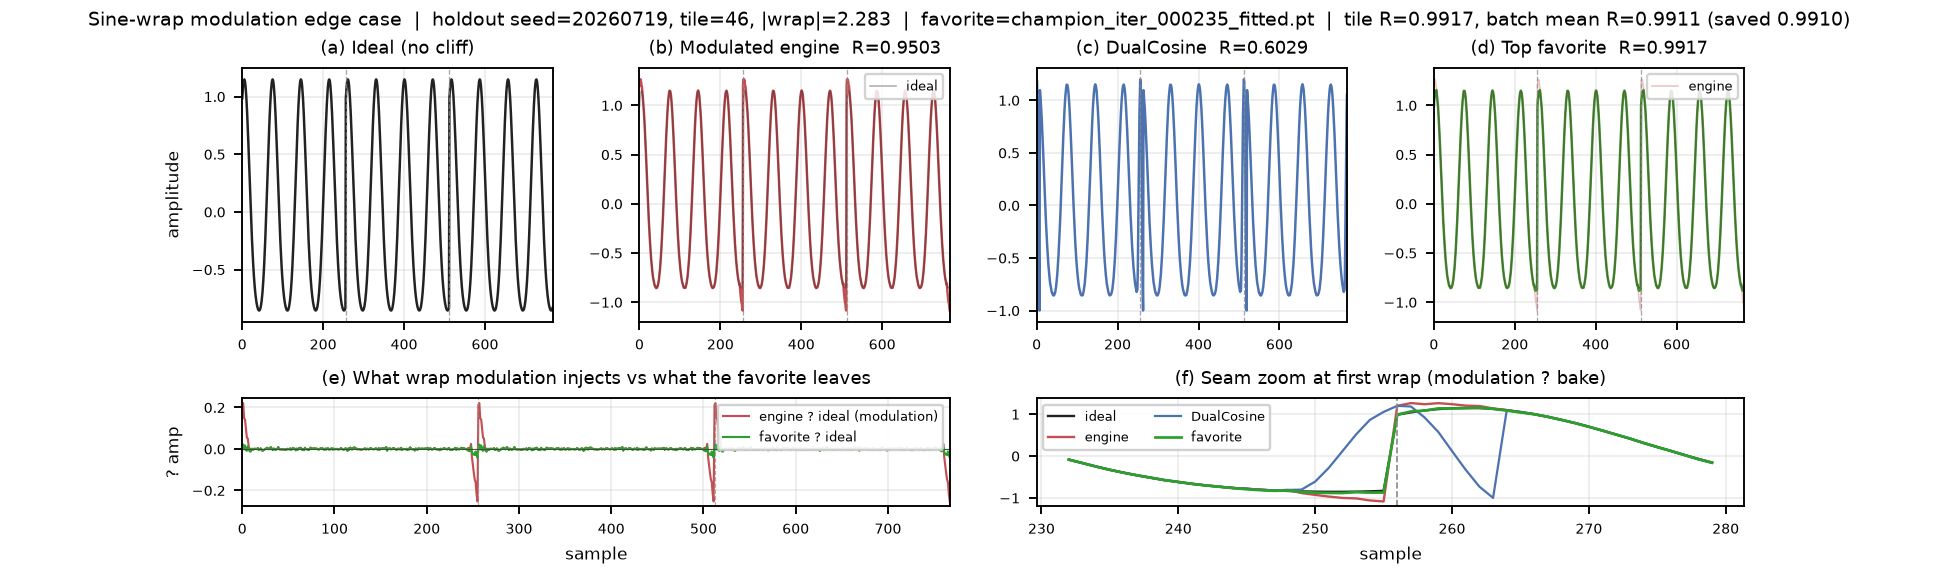
\includegraphics[width=\textwidth]{figures/fig_intro_sine_problem.png}
  \caption{Hard sine-wrap holdout tile (seed~\texttt{20260719}, $L{=}256$, $N{=}16$ tiles; same tile in every panel).
  (a)~Ideal sibling $r^{\star}$ (cliff withheld; scoring target, not a method).
  (b)~No-bake cracked engine $x$ (passthrough $\Theta{=}{\mathrm{id}}$), scored vs~$r^{\star}$.
  (c)~DualCosine classical end fade.
  (d)~Ours (DenoiseOpt favorite bake).
  (e)--(f)~Modulation residual and seam zoom.
  Prolonged residual $R\in[0,1]$ (1~=~best) is printed where scored.}
  \label{fig:intro-sine}
\end{figure*}

Classical virtual-analog tools already address wrap energy locally:
alias-free BLIT/BLEP-style synthesis~\cite{stilson1996}, PolyBLEP / fractional-delay antialiasing~\cite{nam2009polyblep}, and BLAMP corner corrections~\cite{esqueda2016blamp}.
We score cycle-local bake versions of those operators beside DualCosine (Section~\ref{sec:va-seam-baselines}).
The open question is which bake parameters---and which residual cell, if any---minimize tiled error against a no-cliff ideal.

Label-free restoration such as Noise2Noise shows that useful reconstructors can be ranked without paired clean targets when the evaluation geometry is explicit~\cite{lehtinen2018,kashyap2021n2n}.
Mixture-invariant unsupervised separation uses a similar idea for ranking without paired stems~\cite{wisdom2020}.
On the search side, neural architecture search~\cite{elsken2019,zoph2017nas,pham2018}, aging evolution~\cite{real2017large,real2019}, population-based training~\cite{jaderberg2017}, CMA-ES~\cite{hansen2016cmaes}, and evolution-guided policy gradients~\cite{khadka2018} motivate a hybrid outer loop: GA for population diversity, PPO for discrete architecture edits~\cite{schulman2017}, and PBT-style exploit--mutate on elites.
Latency-aware and progressive NAS add compute-aware priors~\cite{tan2019mnasnet,liu2018pnas}.
Mixture-of-experts soft gates suggest routing among small heterogeneous cells under one residual score~\cite{shazeer2017}.
Compact waveform cells draw on Wave-U-Net / Conv-TasNet / dual-path and attention primitives shrunk to bake width~\cite{stoller2018,macartney2018,luo2019,luo2020dprnn,subakan2021,purwins2019,gong2021ast,ronneberger2015,he2016resnet,vaswani2017,jansson2017}.

\paragraph{Noise2Noise baseline and blended score.}
The primary neural comparator is a corrupt$\to$corrupt Noise2Noise seam CNN (\texttt{SeamN2N}, ${\approx}53.5$k parameters) trained on the same generator family~\cite{lehtinen2018,kashyap2021n2n}.
DualCosine stays a classical appendix row and a PPO advantage baseline---not the gate.
Search and champion selection maximize
$J=R_{\mathrm{blend}}-\lambda\cdot\mathrm{latency\_norm}$ with $\lambda{=}0.02$,
where
$R_{\mathrm{blend}}=\alpha R_{\mathrm{seam}}(\mathrm{ideal},\mathrm{out})+(1-\alpha)R_{\mathrm{body}}(\mathrm{eng},\mathrm{out})$
($\alpha{=}0.7$) balances discontinuity-local fidelity against mid-cycle identity
(Section~\ref{sec:residual-score}).
The searchable cell vocabulary includes an explicit \texttt{n2n\_unet} block at SeamN2N-parity scale (distinct from the smaller TinyUNet1D \texttt{unet} block).

\paragraph{Transfer datasets outside wavetables.}
We also score the same wrap protocol on six cycle-local transfer sets
(Section~\ref{sec:transfer-protocol}):
\textbf{CWRU} bearings (drive-end @12\,kHz; cubic ideal vs linear+cliff engine);
\textbf{MFPT} bearings (fixed 25\,Hz shaft; same construction; $n{=}256$ periods);
\textbf{MIT-BIH} Arrhythmia ECG (R--R normal beats with local-mean template ideal);
\textbf{PTB-XL} ECG 500\,Hz subset (PhysioNet \texttt{records500}/\texttt{*\_hr} lead-I windows; subset pilot, not the full corpus);
\textbf{synth CNC G01} (procedural closed-contour residual; KIT CNC login-walled, so synthetic only);
\textbf{synth PMU/AC cycle} (procedural harmonic voltage cycle; IEEE DataPort PMU account-walled, so synthetic only).
Transfer tables compare classical boards unless a deep row is explicitly run.

This paper contributes a meta-search protocol for this periodic seam problem.
An outer RL+GA(+PBT) loop proposes bake-cell graphs and continuous bake parameters.
Each candidate is scored by $R_{\mathrm{blend}}$ (and ranked by $J$) against a procedural ideal sibling $r^{\star}=G(\mathrm{seed},\mathrm{cliff{=}off})$ with body identity vs the cracked engine.
Paired studio-clean wavetables are not required for every trial.
Differentiable DSP modules~\cite{engel2020} place DualCosine / FIR / MLP seam ops in an interpretable stack.
Bayesian HPO~\cite{snoek2012} informs prior families that compete under the same residual geometry.
A CUDA hybrid search campaign (PPO+GA+PBT+NAS, including \texttt{n2n\_unet}) is reported under the v10.1 $R_{\mathrm{blend}}{+}J$ lock in Section~\ref{sec:results}.
Scope is cycle-local wavetable seam restoration (DAFx / AES / arXiv cs.SD).
We do not claim speech enhancement, music source separation, or deep SOTA on classical sci/eng transfer boards.

\subsection{Contributions}
\label{sec:contributions}
\begin{enumerate}
  \item \textbf{Problem framing.} Cast wavetable wrap discontinuity as cycle-local seam restoration under tiled evaluation, with discontinuity-local $R_{\mathrm{seam}}$, mid-cycle body identity $R_{\mathrm{body}}$, and blended primary $R_{\mathrm{blend}}$.
  \item \textbf{Hybrid DenoiseOpt outer loop.} Specify RL+GA(+PBT) search over discrete operator graphs and continuous bake parameters (including SeamN2N-parity \texttt{n2n\_unet}), with named branches and latency-aware objective $J$.
  \item \textbf{Formal residual protocol.} Define bake operator $\Theta$, ideal-sibling generator $G$, outer objective $\max J(R_{\mathrm{blend}},t_{\mathrm{ms}})$, and reimplementable Algorithms~\ref{alg:residual}--\ref{alg:hybrid} (Appendix~\ref{app:algorithms}). No wrap-closure or search-convergence guarantees.
  \item \textbf{Open evaluation path.} Release companion code with frozen N2N gate, balanced ${\approx}1280$-cycle Factory+FX / AKWF / multi-family boards, and named sci/eng transfer benches.
\end{enumerate}

Section~\ref{sec:related_work} organizes related work by mechanism.
Sections~\ref{sec:methods}--\ref{sec:experiments} detail the residual objective and search protocol.
Section~\ref{sec:results} reports the hybrid freeze and inference benches.
